%%%%%%%%%%%%%%%%%%%%%%%%%%%%%%%%%%%%%%%%%%%%%%%%%%%%%%%%%%%%%%%%%%%%%%%%%%%%%%%
%%                                                   FORWARD BACKWARD ASYMMETRY
%%%%%%%%%%%%%%%%%%%%%%%%%%%%%%%%%%%%%%%%%%%%%%%%%%%%%%%%%%%%%%%%%%%%%%%%%%%%%%%
%%                       the chapter about the AFB and the sin2theta extraction



%______________________________________________________________________________
%                     Messung der Asymmetrie und des schwachen Mischungswinkels
\chapter{Messung der Asymmetrie und des schwachen Mischungswinkels}
\label{afb}

\begin{quote}
    The abstact comes last
\end{quote}



%______________________________________________________________________________
%                                                      Datensätze und Selektion
\section{Datensätze und Selektion}
\label{afb:selection}

% + benutzter Datensatz
% + Selektion / Akzeptanz
% + Benutzte Gewichte

% + Kontroll-Plots der Masse / Winkelverteilung / Phi

Die Messung der Vorwärts-Rückwärts Asymmetrie und die anschließende Extraktion
des schwachen Mischungswinkels basiert, wie schon die vorangegangene
Energiekalibration, auf dem vollen Datensatz des Jahres 2012 mit $8\TeV$
Schwerpunktsenergie und einer integrierten Luminosität\footnote{nach Anwendung
der \ac{GRL}} von $20.3\fb^{-1}$. Zur Selektion der interessanten Ereignisse
werden die in Abschnitt \ref{data_sim_selection:selection} beschriebenen
Schnitte angewendet (siehe Tabelle \ref{tab:data_selection}), wobei die
Unterteilung der Ereignismenge nach solchen mit Beteiligung von
Vorwärts-Elektronen (CF) und reinen Zentral-Zentral Ereignissen (CC) zunächst
beibehalten wird. Die Analyse und Messung wird dann in diesen beiden Kanälen
zuerst getrennt durchgeführt und abschließend zu einem kombiniertem Ergebnis
zusammengefasst.
\begin{table} [h]
    \centering
    \begin{tabular}{|l|r|r|}
        \hline
        & \multicolumn{2}{|c|}{Elektronkandidaten}   \\
        \textbf{Schnitt} & \textbf{CC} & \textbf{CF} \\  % escale CF
        \hline\hline
        \ac{GRL}           & 389741202 & 389741202   \\  % 3954702112
        Detektor Status    & 389740981 & 389740981   \\  % 3945153030
        Trigger            & 158129884 & 158129884   \\  % 1402546381
        primärer Vertex    & 157901943 & 157901943   \\  % 1400899527
        Pseudorapidität    & 149728397 & 122396071   \\  % 1328016208
        Transversal-Impuls &  63811039 &   8342860   \\  %  498956943
        Autor              &  17186000 &   7841721   \\  %  378463236
        ID                 &   4326530 &    995073   \\  %   76603185
        Ladung             &   4266425 &  (995073)   \\  %           
        OQ                 &   4245028 &    988991   \\  %   75178238
        \hline
    \end{tabular}
    \caption[Anzahl der Elektronkandidaten in Daten für CC und CF Selektion]
        {Anzahl der Elektronkandidaten in Daten nach für CC und CF Selektion.
        Die Auflistung ist inklusiv, d.h. untere Schnitte enthalten implizit
        alle vorangegangenen Schnitte. \development (check numbers with
        calibration)}
    \label{tab:data_selection}
\end{table}
Auf alle Elektronkandidaten im Datensatz werden zuvor noch die entsprechenden
Kalibrationfaktoren für die Energie angewendet (siehe Kapitel
\ref{data_sim_selection:data} und \ref{energy_calibration}), sodass die
Selektion auf kalibrierten Energiewerten stattfinden kann.

Zur simulationsseitigen Beschreibung des Signalprozesses
$pp \rightarrow \gamma^*/Z(e^+e^-) + X$, also dem elektroschwachen Zerfall
eines $Z$-Bosons bzw. virtuellen Photons in ein Elektronpaar\footnote{auch hier
wird der Begriff \textit{Elektron} wieder synonym für Teilchen und Antiteilchen
verwendet}, wird das von \textsc{Powheg+Pythia} generierte Drell-Yan
Monte-Carlo verwendet (siehe Kapitel \ref{used_mc_samples}). Es werden
identische Selektionkriterien, wie auf den Daten angewendet, wobei die Energie
der Elektronkandidaten zuvor einer Auflösungskorrektur unterzogen wird. Dabei
wird eine künstliche Verschmierung der Energie eingeführt, um die oftmals zu
optimistisch angenommene Energieauflösung im Monte-Carlo nachträglich zu
korrigieren\footnote{weitere Details siehe Kapitel \ref{energy_calibration}}.
Zudem wird für jedes selektierte Ereigniss ein spezifisches Gewicht errechnet,
mit dem dieses Ereignis bei der Erstellung von statistischen Verteilungen
beträgt. Es gehen hierbei Ereignis spezifische, sowie Elektron spezifische
Korrekturfaktoren in die Bildung dieses Gewichtes ein, deren Ursprung und
Benutzung in Kapitel \ref{mc_corrections} motiviert wurde. Zusammengefasst
ergeben sich die Gesamtgewichte zu
\begin{align}
    w_\text{event}^\text{CC} &= w_\text{pu} \cdot w_\text{kFactor} \cdot
        w_\text{vtx} \cdot w_\text{gen} \cdot \prod_{i=1,2} w_{\text{ID},i}
        \cdot w_{\text{spur},i} \cdot w_{\text{trigger},i}
        \\[2pt]
    w_\text{event}^\text{CF} &= w_\text{pu} \cdot w_\text{kFactor} \cdot
        w_\text{vtx} \cdot w_\text{gen} \cdot w_{\text{ID},1} \cdot
        w_{\text{ID},2} \cdot w_{\text{spur}} \cdot w_{\text{trigger}}
\end{align}
wobei der Index $i$ in \ac{CC} Ereignissen verdeutlicht, dass die
entsprechenden Korrekturfaktoren für beide Zentral-Elektronen separat eingehen.
In \ac{CF} Ereignissen findet diese Unterscheidung nur für den Faktor der
Identifikationseffizienz statt, da die beiden übrigen Effizienzkorrekturen
nicht für Vorwärts-Elektronen definiert sind.

Zur Abschätzung der Beiträge von Untergrundprozessen wird eine Kombination aus
Simulation und datengestützter Betimmung verwendet. Beide Aspekte werden im
Folgenden näher erläutert und deren Anteil an den selektierten Ereignissen
quantifiziert.



\subsection{Simulierte Untergrundbeiträge}
\label{afb:monte_carlos}

% + Benutzte Monte-Carlos

Neben dem Drell-Yan Prozess mit zwei Elektronen im Endzustand gibt es
zahlreiche weitere Prozesse, die eine ähnliche Signatur im Detektor zeigen und
deshalb von der oben beschriebenen Selektion inkludiert werden. Das Prinzip der
Abschätzung dieser Untergrundbeiträge mittels Simulationen, beruht auf der
Erstellung von Monte-Carlos für jeden relevanten, d.h. möglicherweise
beitragenden, Prozess und der anschließenden Anwendung der selben
Selektionsschnitte, analog zur Selektion in realen Daten. Die aus den
verbleibenden Ereignissen gewonnenen Verteilungen\footnote{Selbstverständlich
ist hierbei auch die mit Gleichung (\ref{eq:mc_scaling}) beschriebene
Skalierung auf Luminosität erforderlich} quantifizieren sodann den Beitrag des
jeweilig betrachteten Prozesses. Alle hier nachstehend aufgeführten Monte-Carlo
Simulationen sind mit ihren Charakteristika bereits in Kapitel
\ref{used_mc_samples} eingeführt worden und werden hier vom motivierenden
Standpunkt der Untergrundabschätzung aus betrachtet.

Einen der größten Beiträge zum Untergrund stellt die Produktion und der Zerfall
eines Top-Antitop Quarkpaares dar (im Folgenden mit \texttt{ttbar} bezeichnet).
Topquarks haben ein Verzweigungsverhältnis von beinahe 100\% für den Zerfall in
ein $b$-Quark und ein $W$-Boson. Solche Ereignisse passieren die Selektion,
wenn entweder beide $W$-Bosonen leptonisch in jeweils ein Elektron und ein
Antielektronneutrino zerfallen, oder Jets aus den $b$-Quarks bzw. dem
hadronischen Zefall eines oder beider $W$-Bosonen fälschlicherweise als
Elektronen rekonstruiert werden. Ähnlich, jedoch in sehr viel geringerem
Umfang, trägt auch die Produktion eines einzelnen Top-Quarks und dessen
konsekutiver Zerfall zum Untergrund bei (nachfolgend \texttt{SingleTop}
genannt). Die relevanten Zerfallskanäle sind dieselben, jedoch muss nun
folgerichtig stets ein irrtümlich identifizierter Jet beteiligt sein.

Der leptonische Zerfall eines $W$-Bosons in ein Elektron und ein
Antielektronneutrino spielt auch für sich allein betrachtet eine wichtige
Rolle. Der Wirkungsquerschnitt für die Produktion eines $W$-Bosons ist um
einiges größer, als für den untersuchten Signal-Prozess. Wie schon beim
Topquark-Untergrund tragen hier Ereignisse bei, in denen ein Jet von den
Rekonstruktionsalgorithmen als Elektron erkannt wird. Auch der verwandte
Prozess des $W$-Zerfalls in ein Tauon und das entsprechende Antineutrino
liefern einen Beitrag, da Tauonen eine Verzweigungsverhältnis von rund $18\%$
für den Zerfall in ein Elektron aufweisen. Zusammengefasst werden alle
Untergründe dieser Art in der Folge mit \texttt{WJets} gekennzeichnet.

Ein weitere Kontribution zum Untergrund entstammt der Produktion von $WW$-,
$WZ$- und $ZZ$-Bosonpaaren. Hier finden sich im Endzustand häufig zwei oder
Elektronen, sodass die Wahrscheinlichkeit hoch ist, dass diese die
kinematischen Anforderungen erfüllen und sie Selektion passieren können.
Natürlich kommen hierbei auch wieder falsch identifizierte Jets aus
hadronischen Zerfällen zum Tragen. Im folgenden werden aber alle Prozesse
dieser Art, also solche, die die Produktion eines der genannten Bosonpaare
beinhalten, unter dem Begriff \texttt{Diboson} zusammengefasst.

Einen sehr geringen, wenn auch nicht vernachlässigbaren Anteil liefert der
Drell-Yan Prozess selbst, nämlich beim Zerfall in ein $\tau^+\tau^-$-Paar
(\texttt{DYtautau}). Wie schon beim $W$-Untergrund erwähnt können Tauonen in
Elektronen zerfallen, weshalb dieser Prozess in der Lage ist, von der Selektion
erfasst zu werden.

Abbildung \ref{fig:elec_kinematics} zeigen die
Verteilungen des Transversalimpulses $p_T$ und der Pseudorapidität $\eta$ für
die einzelnen Elektronen nach Anwendung der Selektionsschnitte. Die
Untergrundbeiträge sind entsprechend der oben eingeführten Kürzel
(\texttt{ttbar},...) farbig gekennzeichnet und aufeinandergestapelt
dargestellt.

\begin{figure}[h]
    \centering
    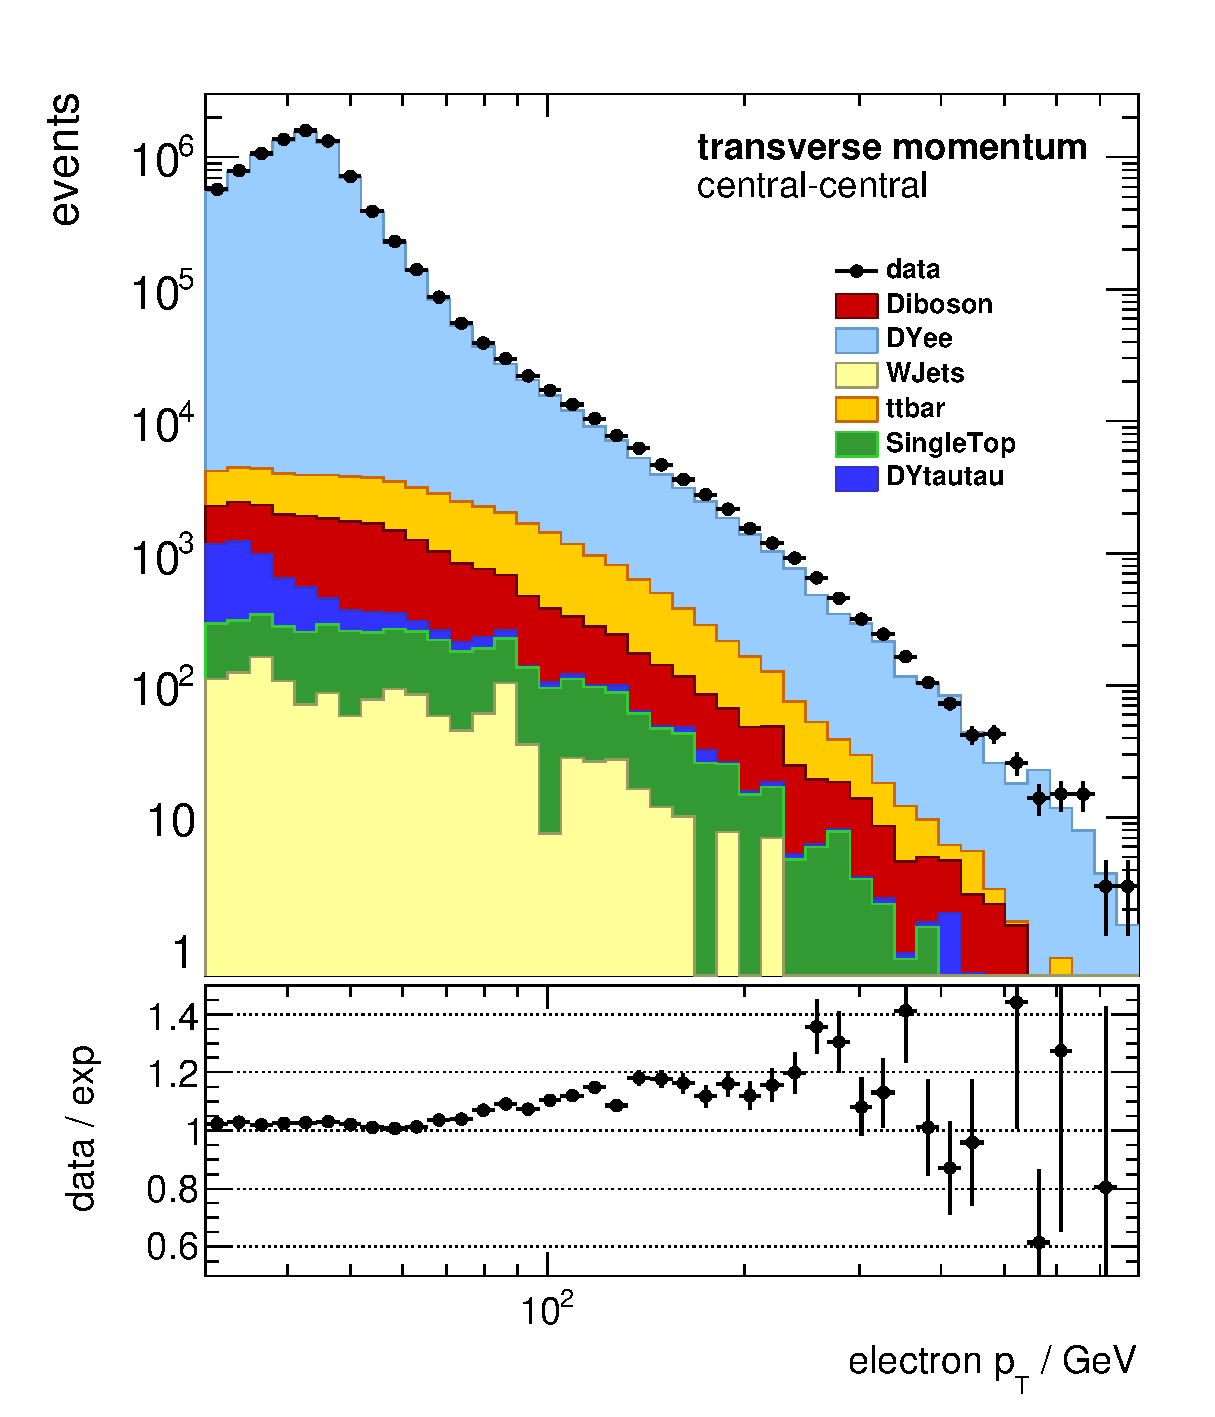
\includegraphics[width=0.48\textwidth]{plots/pt_cc}
    \hfill
    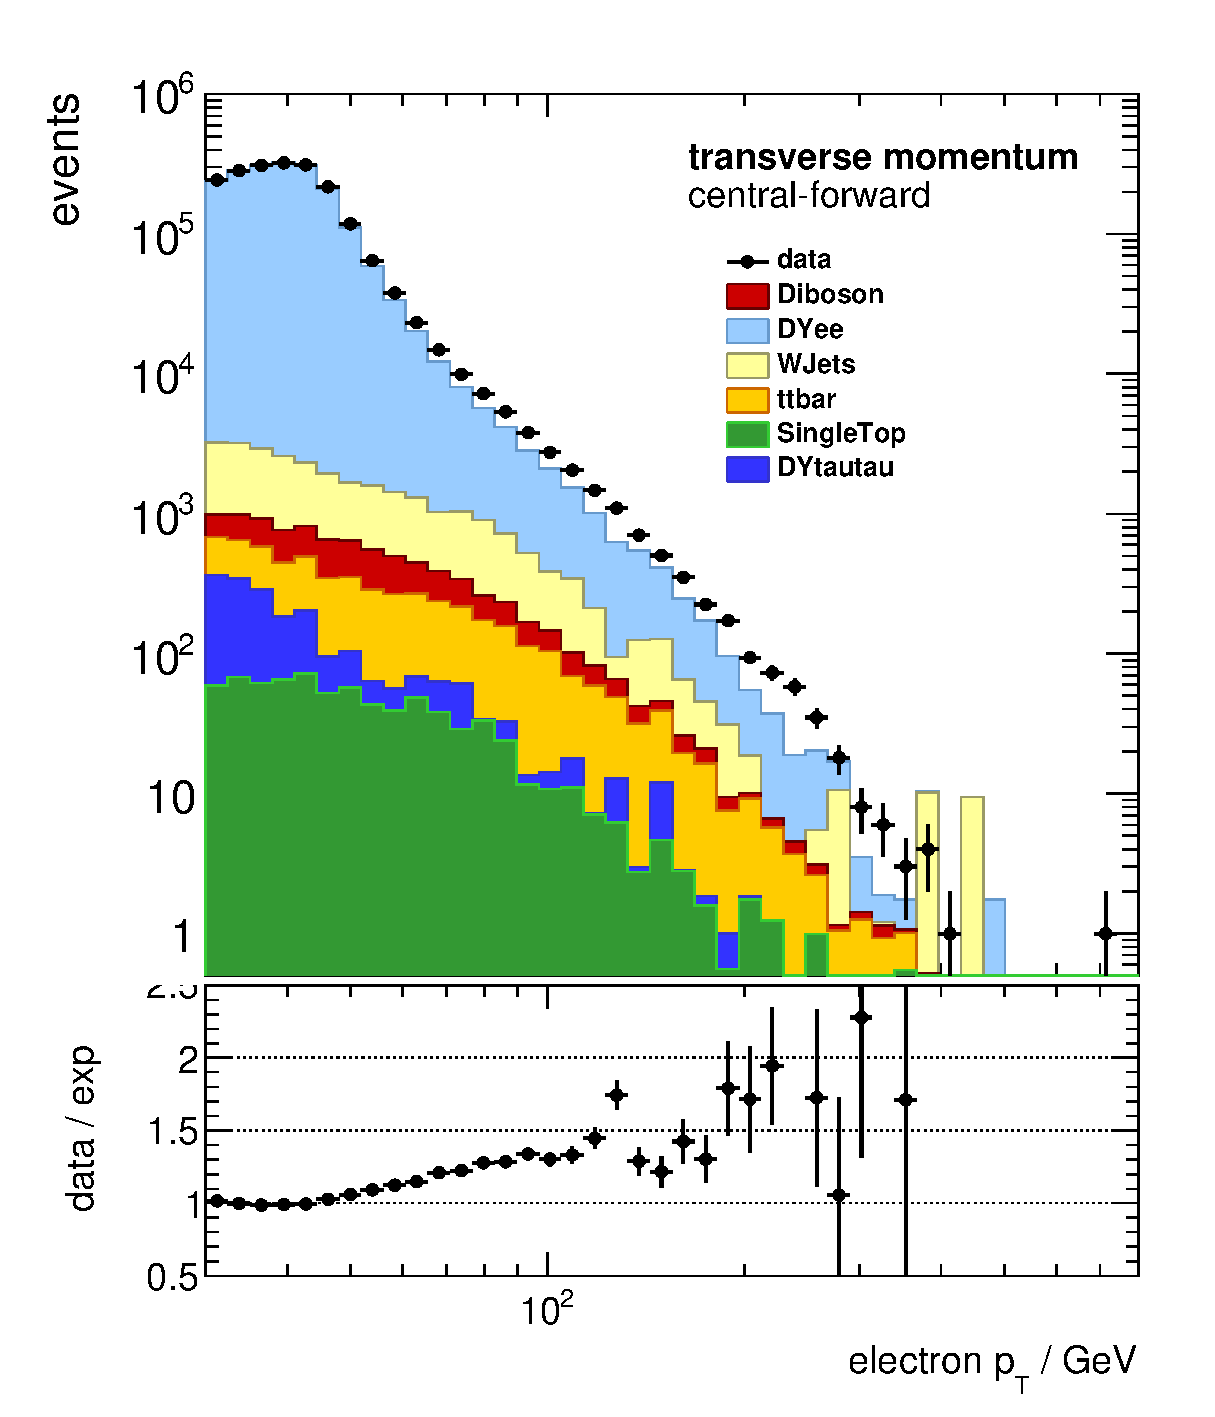
\includegraphics[width=0.48\textwidth]{plots/pt_cf}

    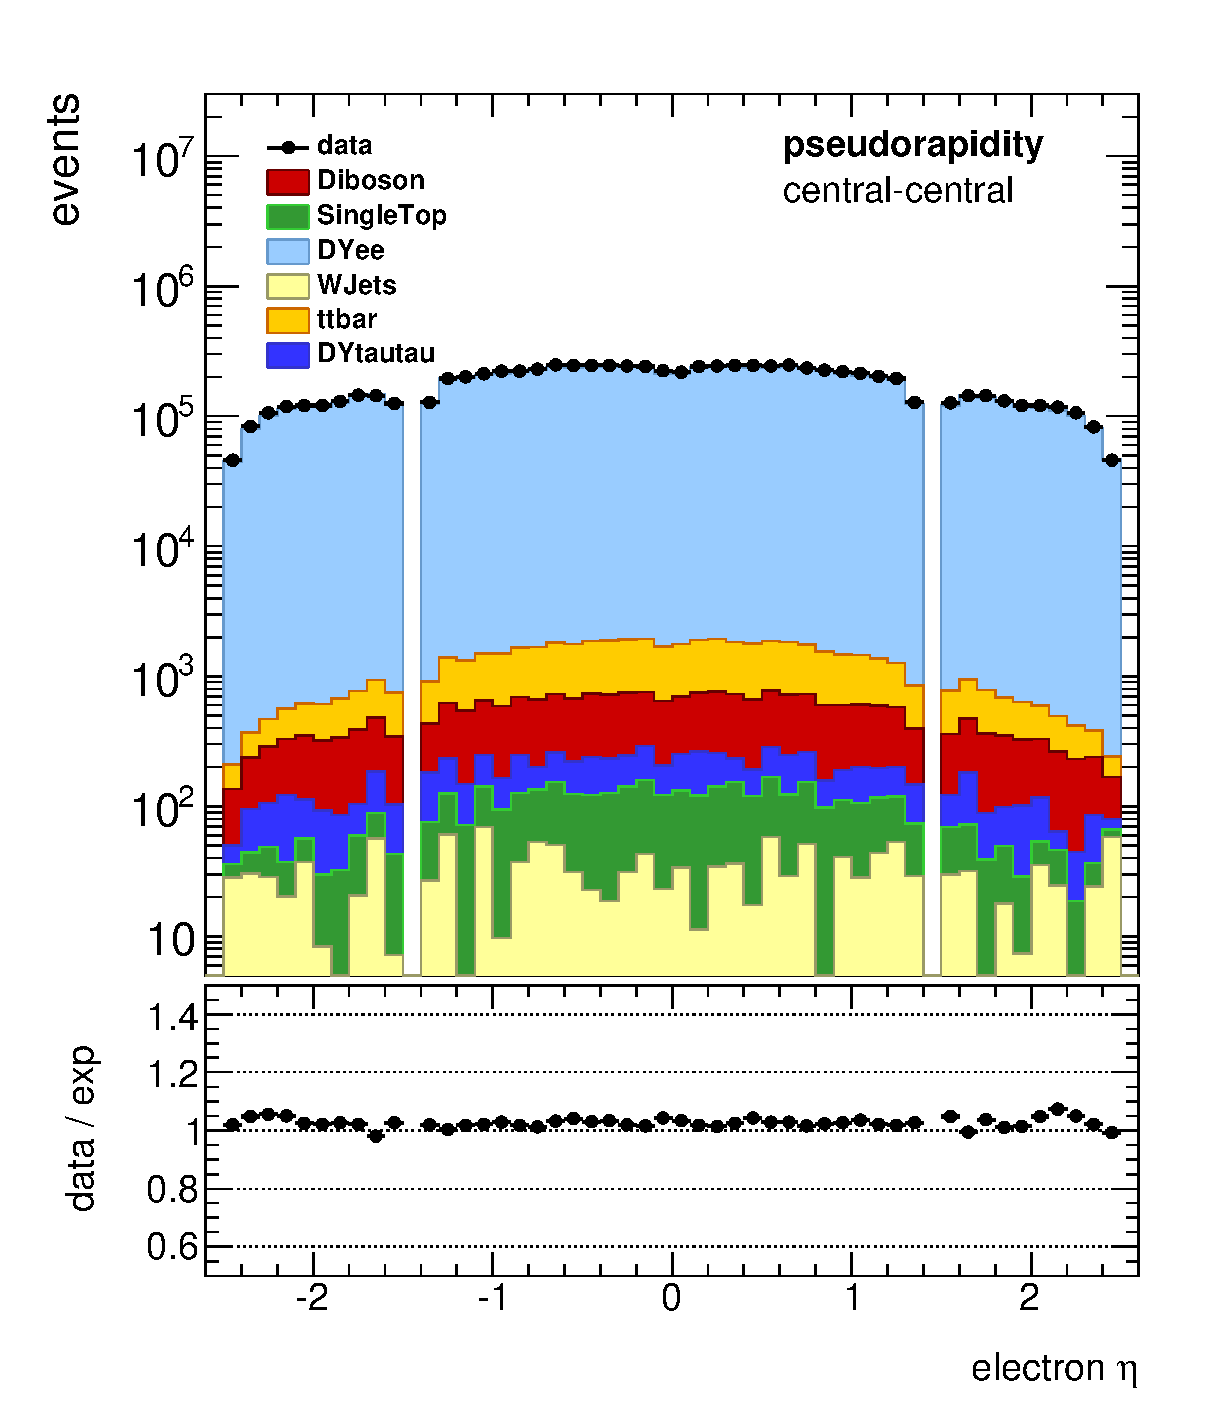
\includegraphics[width=0.48\textwidth]{plots/eta_cc}
    \hfill
    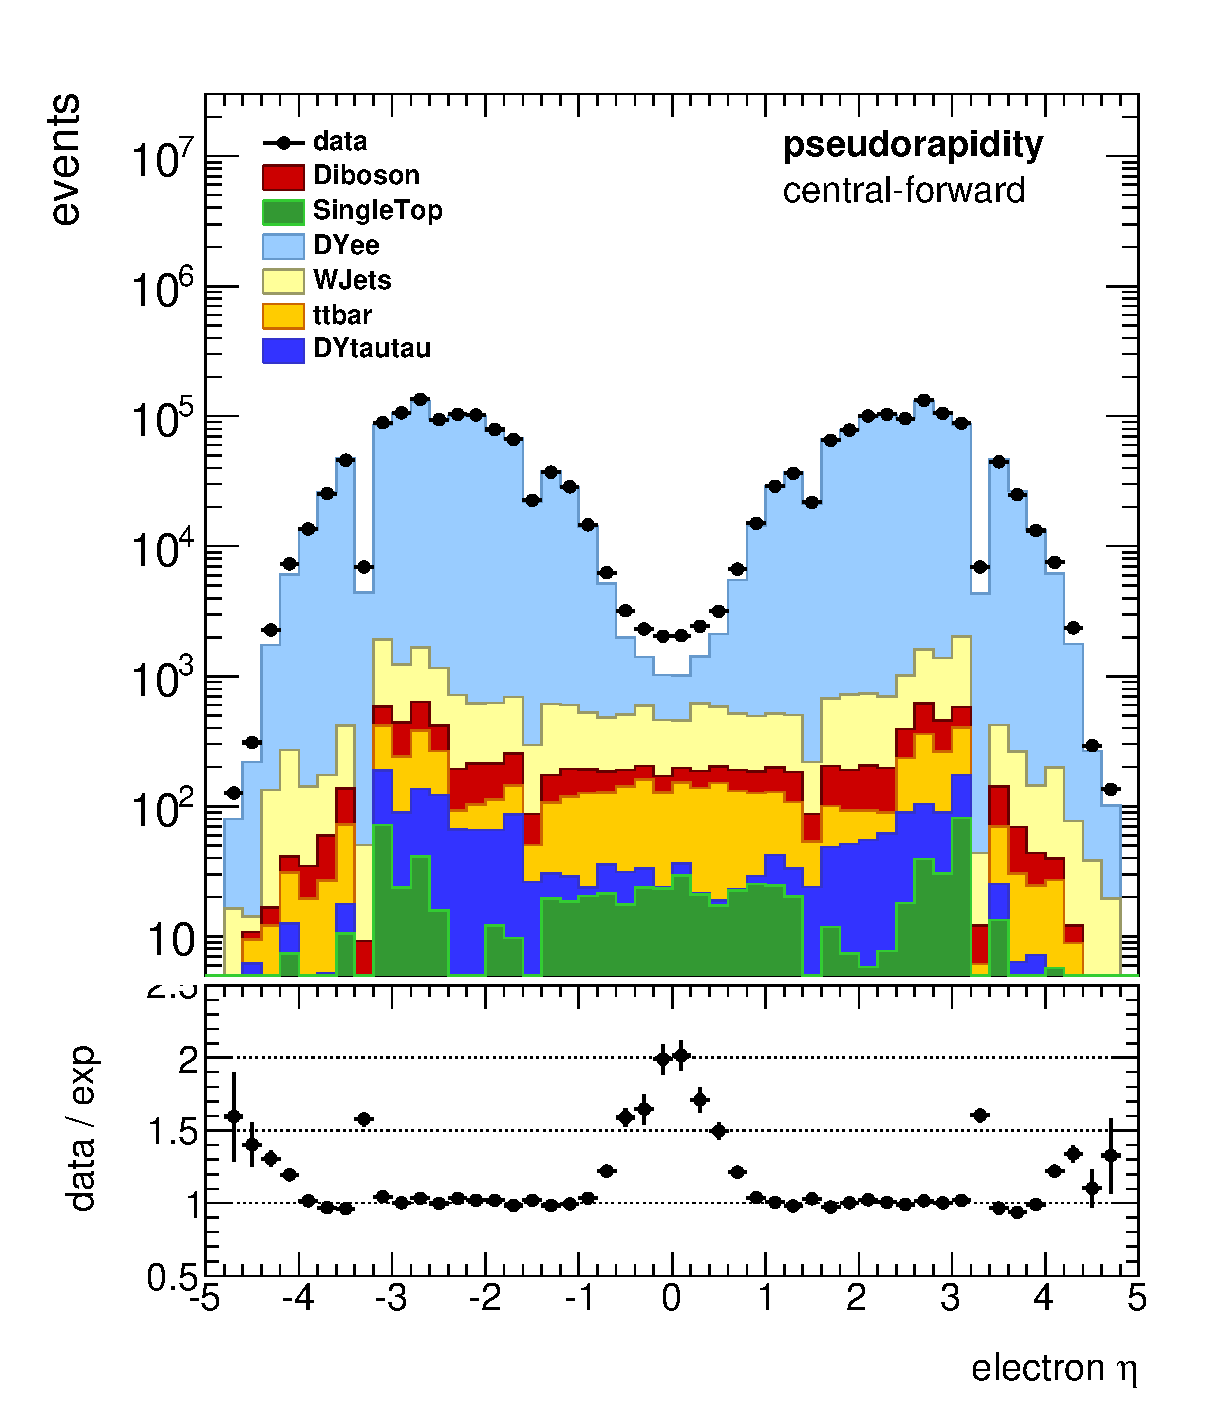
\includegraphics[width=0.48\textwidth]{plots/eta_cf}
    \caption[Kinematische Verteilungen der Elektronen nach Selektion in \ac{CC}
        und \ac{CF}]
        {Kinematische Verteilungen der Elektronen nach Selektion in \ac{CC}
        (links) und \ac{CF} (rechts) für den Transversalimpuls (oben) und die
        Pseudorapidität (unten). Der Quotient aus Daten und dargestellter
        Untergundsumme ist jeweils unter den Histogrammen gezeigt.}
    \label{fig:elec_kinematics}
\end{figure}

Erwartungsgemäß zeigen die Verteilungen des Transversalimpulses in Daten ein
Maximum bei etwa $45\GeV$, also gerade der halben Masse des $Z$-Bosons
und einen daran anschließenden starken Abfall mit steigendem Transversalimpuls.
Ein analoges Verhalten wird bei der Simulation des Signalprozesses
(\texttt{DYee}) beobachtet. Die übrigen Untergrundspektren weisen ebenfalls den
erwarteten Verlauf eines mit größer werdendem $p_T$ abfallendes Spektrum auf,
zeigen dagegen aber keine ausgeprägte Extremstelle. Einzige Ausnahme stellt das
\texttt{DYtautau} Spektrum dar, welches ein solches Maximum unterhalb von
$45\GeV$ aufweist. Die Verschiebung dieses Maximums unter die halbe $Z$-Masse
liegt darin begründet, dass die Elektronen in diesem Prozess aus den
direkten Zerfallsprodukten des Bosons, also den Tauonen, hervorgehen und
folglich  nicht deren vollen Impuls tragen.

Desweiteren fällt beim Vergleich zwischen den Spektren für \ac{CC}- und
\ac{CF}-Selektion auf, dass sich der Umfang der Untergrundbeiträge deutlich 
unterscheidet. Am deutlichsten zeigt sich dies beim \texttt{WJets}
Untergrund, der in \ac{CF} den größten Beitrag zum Untergrund darstellt,
während dessen Beitrag in \ac{CC} eine untergeordnete Rolle spielt. Die Ursache
hierfür ist, dass im Vorwärts-Bereich die Wahrscheinlichkeit der
Fehlidentifikation eines Jets als Elektron wesentlich höher ist, als im
Zentral-Bereich, was unter anderem auf die fehlende Spurinformation im
Vorwärts-Bereich zurückzuführen ist\footnote{siehe hierzu auch Kapitel \ref{}}.

Unter jeder Abbildung ist zudem der Quotient aus der Datenverteilung und der
Summe alle Monte-Carlos (Untergründe + Signal) dargestellt. Diese zeigt, gerade
in Bereichen mit hohem Transversalimpuls eine deutliche Diskrepanz. Hierin
verbirgt sich ein weiterer fehlender Untergundbeitrag der durch Prozesse der
\ac{QCD} bestimmt ist und deshalb nur schwer simulierbar ist. Die Methode zur
Abschätzung dieses Beitrags ist Gegenstand des nachfolgenden Abschnitts.

Bei der Betrachtung der Spektren der Pseudorapidität ist zu beachten, dass
diese auf unterschiedlichen Skalen, entsprechend der jeweiligen Schnitte in der
Selektion, aufgetragen sind. Die Form der Verteilungen in Daten zeigen im
\ac{CC} Kanal einen leicht nach außen abfallenden Verlauf, während im \ac{CF}
Kanal zwei deutliche symmetrische Erhebungen auszumachen sind. Dies ist den
angewendeten Selektionkriterien geschuldet, die den Öffnungswinkel zwischen den
beiden Elektronen gerade in der \ac{CF}-Selektion einschränken. 




\subsection{Datengestützte Untergrundabschätzung}
\label{afb:multijet}

% + MultiJet-Untergrund Bestimmung







%______________________________________________________________________________
%                                                         Asymmetrie Verteilung
\section{Vorwärts-Rückwärts Asymmetrie Verteilung}
\label{afb:afb}

% + Rohe Verteilung
% + Untergund reduzierte Verteilung
% + Vergleich mit Signal-Simulation



%______________________________________________________________________________
%                          Extraktion des effektiven Schwachen Mischungswinkels
\section{Extraktion des effektiven Schwachen Mischungswinkels}
\label{afb:sin2theta}

% + Extraktionsmethode
%   - Template Erzeugung
%   - Faltung mit Detektoreffekten
% + Extraktion
%   - Template Fits
%   - Closure-Test
%   - Resultate (einzeln und kombiniert)
% + Diskussion
%   - Systematische Betrachtungen
%   - Vergleich mit anderen Experimenten
%   - Ausblick
 


